\documentclass[a4paper]{article}
\usepackage[english]{babel}
\usepackage{setspace}
\usepackage{mathtools}
\usepackage{listings}
\usepackage{ulem}
\usepackage[utf8]{inputenc}
\usepackage{eurosym}
\usepackage{fancyhdr}
\usepackage{tikz}
\usetikzlibrary{calc}
\usetikzlibrary{positioning}
\usetikzlibrary{arrows.meta}
\usetikzlibrary{fit}
\usepackage{tikzscale}
\usepackage{wrapfig}
\setcounter{secnumdepth}{-1}
\pagestyle{fancy}
\fancyhf{}
\setlength{\headheight}{24.0pt}
\lhead{Multi-Agent Systems,  Winter Semester 2018/2019, Exercise 1\\
       Submitted by: Amadeus Hovekamp, Hans Nübel, Jonathan Pieper}
\cfoot{\thepage}

\usepackage[
        colorlinks = true,    % Disable drawing boxes around links.
        linkcolor = black,    % Sets the color of links to black.
    ]{hyperref}
\newcommand{\refequation}[1]{\hyperref[#1]{(\ref{#1})}}

\begin{document}
\title{Exercise Sheet 1: Solution}
\author{}
\date{\today}
\section{Exercise 1.1}
\subsection{a)}
Each clause is a disjunction containing at least one negated atom. Therefore, the interpretation $p_i \mapsto T \quad \forall i$ satisfies S.
\subsection{b)}
\begin{align*}
&(p \land (q \lor \lnot p))\lor(r \land \lnot(s \lor r)) \quad& \text{ Commutativity}\\
\implies&(p \land (\lnot p \lor q))\lor(r \land \lnot(r \lor s)) & \text{De Morgan}\\
\implies&(p \land (\lnot p \lor q))\lor(r \land \lnot r \land \lnot s)) & \text{Contradiction}\\
\implies&(p \land (\lnot p \lor q))\lor(\bot \land \lnot s)) & \text{Falsity}\\
\implies&(p \land (\lnot p \lor q))\lor\bot & \text{Falsity}\\
\implies& p \land (\lnot p \lor q) & \text{Distributivity}\\
\implies&(p \land \lnot p) \lor (p \land q) & \text{Contradiction}\\
\implies&\bot \lor (p \land q) & \text{Falsity}\\
\implies& p \land q & \\
\end{align*}
\section{Exercise 1.2}
\subsection{a)}
\begin{tikzpicture}[level distance=10mm,sibling distance=5em,every node/.style = {align=center}]
\node {$(p \rightarrow q) \land (p \lor r) \land \lnot q$}
    child { node {$p \rightarrow q$}
        child { node {$p \lor r$}
            child { node (a1) {$\lnot q$}
                child { node (b1) {$\lnot p$}
                    child { node (b2) {$p$}}
                    child { node {$r$}}}
                child { node (a2) {$q$}
}}}};
\draw [<->, dashed] (a1.east) to [bend left] (a2.north);
\draw [<->, dashed] (b1.west) to [bend right] (b2.north);
\end{tikzpicture}\\\\
All branches are either saturated or closed. The only open branch provides the model
$p \mapsto F, q \mapsto F, r \mapsto T$.
\subsection{b)}
\begin{tikzpicture}[level distance=10mm,sibling distance=5em,every node/.style = {align=center}]
\node {$\lnot ((\lnot p\land q \land r) \lor (p \land q) \lor (\lnot p \land \lnot r) \lor \lnot q)$}
        child { node {$p \lor \lnot q \lor \lnot r$}
            child { node { $\lnot p \lor \lnot q$}
                child { node { $p \lor r$}
                    child { node (a1) {$q$}
                        child { node (b1) {$p$}
                            child { node (b2) {$\lnot p$}}
                            child { node (b3) {$\lnot q$}}}
                        child { node (a2) {$\lnot q$}}
                        child { node (c1) {$\lnot r$}
                            child { node (d1) {$\lnot p$}
                                child{ node (d2) {$p$}}
                                child{ node (c2) {$r$}}}
                            child { node (a3) {$\lnot q$}}}
}}}};
\draw [<->, dashed] (a1.south east) to [bend left] (a2.north east);
\draw [<->, dashed] (a1.east) ++(0, 0.2em) to [bend left] (a3.north);
\draw [<->, dashed] (b1.west) to [bend right] (b2.north);
\draw [<->, dashed] (a1.south west) to (b3.north);
\draw [<->, dashed] (c1.south) to (c2.north);
\draw [<->, dashed] (d1.west) to [bend right] (d2.north);
\end{tikzpicture}\\\\
Since its negation is unsatisfiable, $(\lnot p\land q \land r) \lor (p \land q) \lor (\lnot p \land \lnot r) \lor \lnot q$ is a tautology.
\subsection{c)}
\begin{tikzpicture}[level distance=10mm,sibling distance=5em,every node/.style = {align=center},
level 5/.style={sibling distance=10em},
level 6/.style={sibling distance=5em}]
\node {$p \land \lnot q \land (r \land p) \rightarrow (q \lor \lnot r) \land r$}
    child { node (a1) {$p$}
        child { node (b1) {$\lnot q$}
            child { node {$(r \land p) \rightarrow (q \lor \lnot r)$}
                child { node (c1) {$r$}
                    child { node {$\lnot (r \land p)$}
                        child{ node (a2) {$\lnot p$}}
                        child{ node (c2) {$\lnot r$}}}
                    child { node {$(q \lor \lnot r)$}
                        child{ node (c3) {$\lnot r$}}
                        child{ node (b2) {$q$}}}
}}}};
\draw [<->, dashed] (a1.west) to [bend right] (a2.north);
\draw [<->, dashed] (b1.east) to [bend left] (b2.north);
\draw [<->, dashed] (c1.south west) ++(0.3em, 0) to (c2.north);
\draw [<->, dashed] (c1.south east) ++(-0.3em, 0) to (c3.north);
\end{tikzpicture}\\\\
$p \land \lnot q \land (r \land p) \rightarrow (q \lor \lnot r) \land r$ is unsatisfiable, therefore\\
$\{p \land \lnot q, (r \land p) \rightarrow (q \lor \lnot r)\} \models \lnot r$

\pagebreak


\section{Exercise 1.3}

Detailed transformations for the first statement, with $C$ meaning that Cyclope is guilty and
$\lnot C$ that Cyclope is not guilty. Other abbreviations analogous.


\begin{equation*}
\begin{aligned}
           & & \left( \lnot C \land E \land \lnot A \right) \lor \left( C \land \lnot \left( E \land \lnot A \right) \right) \\
    \equiv & & \left( \lnot C \land E \land \lnot A \right) \lor \left( C \land \left( \lnot E \lor A \right) \right) \\
    \equiv & & \left( \lnot C \lor \left( C \land \left( \lnot E \lor A \right) \right) \right)
               \land \left( E \lor \left( C \land \left( \lnot E \lor A \right) \right) \right)
               \land \left( \lnot A \lor \left( C \land \left( \lnot E \lor A \right) \right) \right) \\
    \equiv & & \left( \lnot C \lor C \right) \land \left( \lnot C \lor \lnot E \lor A \right)
               \land \left( E \lor C \right) \land \left( E \lor \lnot E \lor A \right)
               \land \left( \lnot A \lor C \right) \land \left( \lnot A \lor \lnot E \lor A \right) \\
    \equiv & & \left( \lnot C \lor \lnot E \lor A \right) \land \left( E \lor C \right) \land \left( \lnot A \lor C \right)
\end{aligned}
\end{equation*}

This leads to the following set of formulae (applying the steps above to all statements):

\begin{equation}
 \left\{ \lnot C , \lnot E , A \right\} \tag{1.1} \label{1.1}
\end{equation}
\begin{equation}
\left\{ C , E \right\} \tag{1.2} \label{1.2}
\end{equation}
\begin{equation}
\left\{ C , \lnot A \right\} \tag{1.3} \label{1.3}
\end{equation}

\begin{equation}
 \left\{ \lnot E , \lnot G , \lnot L \right\} \tag{2.1} \label{2.1}
\end{equation}
\begin{equation}
\left\{ E , G \right\} \tag{2.2} \label{2.2}
\end{equation}
\begin{equation}
\left\{ E , L \right\} \tag{2.3} \label{2.3}
\end{equation}

\begin{equation}
 \left\{ \lnot A , \lnot Sh , L \right\} \tag{3.1} \label{3.1}
\end{equation}
\begin{equation}
\left\{ A , Sh \right\} \tag{3.2} \label{3.2}
\end{equation}
\begin{equation}
\left\{ A , \lnot L \right\} \tag{3.3} \label{3.3}
\end{equation}

\begin{equation}
 \left\{ \lnot G , \lnot W , P \right\} \tag{4.1} \label{4.1}
\end{equation}
\begin{equation}
\left\{ G , W \right\} \tag{4.2} \label{4.2}
\end{equation}
\begin{equation}
\left\{ G , \lnot P \right\} \tag{4.3} \label{4.3}
\end{equation}

\begin{equation}
 \left\{ \lnot I , E , St \right\} \tag{5.1} \label{5.1}
\end{equation}
\begin{equation}
\left\{ I , \lnot E \right\} \tag{5.2} \label{5.2}
\end{equation}
\begin{equation}
\left\{ I , \lnot St \right\} \tag{5.3} \label{5.3}
\end{equation}

\begin{equation}
 \left\{ \lnot L , \lnot I , W \right\} \tag{6.1} \label{6.1}
\end{equation}
\begin{equation}
\left\{ L , I \right\} \tag{6.2} \label{6.2}
\end{equation}
\begin{equation}
\left\{ L , \lnot W \right\} \tag{6.3} \label{6.3}
\end{equation}

\begin{equation}
 \left\{ \lnot M , \lnot P , C \right\} \tag{7.1} \label{7.1}
\end{equation}
\begin{equation}
\left\{ M , P \right\} \tag{7.2} \label{7.2}
\end{equation}
\begin{equation}
\left\{ M , \lnot C \right\} \tag{7.3} \label{7.3}
\end{equation}

\begin{equation}
 \left\{ \lnot P , \lnot E , \lnot G \right\} \tag{8.1} \label{8.1}
\end{equation}
\begin{equation}
\left\{ P , E \right\} \tag{8.2} \label{8.2}
\end{equation}
\begin{equation}
\left\{ P , G \right\} \tag{8.3} \label{8.3}
\end{equation}

\begin{equation}
 \left\{ \lnot Sh , \lnot C , I \right\} \tag{9.1} \label{9.1}
\end{equation}
\begin{equation}
\left\{ Sh , C \right\} \tag{9.2} \label{9.2}
\end{equation}
\begin{equation}
\left\{ Sh , \lnot I \right\} \tag{9.3} \label{9.3}
\end{equation}

\begin{equation}
 \left\{ \lnot St , \lnot G , M \right\} \tag{10.1} \label{10.1}
\end{equation}
\begin{equation}
\left\{ St , G \right\} \tag{10.2} \label{10.2}
\end{equation}
\begin{equation}
\left\{ St , \lnot M \right\} \tag{10.3} \label{10.3}
\end{equation}

\begin{equation}
 \left\{ \lnot V , \lnot M , Sh \right\} \tag{11.1} \label{11.1}
\end{equation}
\begin{equation}
\left\{ V , M \right\} \tag{11.2} \label{11.2}
\end{equation}
\begin{equation}
\left\{ V , \lnot Sh \right\} \tag{11.3} \label{11.3}
\end{equation}

\begin{equation}
 \left\{ \lnot W , \lnot St , \lnot V \right\} \tag{12.1} \label{12.1}
\end{equation}
\begin{equation}
\left\{ W , St \right\} \tag{12.2} \label{12.2}
\end{equation}
\begin{equation}
\left\{ W , V \right\} \tag{12.3} \label{12.3}
\end{equation}

Now apply resolution:

\begin{equation}
\refequation{1.2} + \refequation{8.1}: \  \ \left\{ C , \lnot P , \lnot G \right\} \tag{13} \label{13}
\end{equation}

\begin{equation}
\refequation{4.3} + \refequation{13}: \  \ \left\{ C , \lnot P \right\} \tag{14} \label{14}
\end{equation}

\begin{equation}
\refequation{7.2} + \refequation{14}: \  \ \left\{ C , M \right\} \tag{15} \label{15}
\end{equation}

\begin{equation}
\refequation{7.3} + \refequation{15}: \  \ \left\{ M \right\} \tag{16} \label{16}
\end{equation}

\begin{equation}
\refequation{10.3} + \refequation{16}: \  \ \left\{ St \right\} \tag{17} \label{17}
\end{equation}

\begin{equation}
\refequation{5.3} + \refequation{17}: \  \ \left\{ I \right\} \tag{18} \label{18}
\end{equation}

\begin{equation}
\refequation{9.3} + \refequation{18}: \  \ \left\{ Sh \right\} \tag{19} \label{19}
\end{equation}

\begin{equation}
\refequation{11.1} + \refequation{19}: \  \ \left\{ V \right\} \tag{20} \label{20}
\end{equation}

\begin{equation}
\refequation{12.1} + \refequation{20}: \  \ \left\{ \lnot W , \lnot St \right\} \tag{21} \label{21}
\end{equation}

\begin{equation}
\refequation{17} + \refequation{21}: \  \ \left\{ \lnot W \right\} \tag{22} \label{22}
\end{equation}

\begin{equation}
\refequation{6.1} + \refequation{22}: \  \ \left\{ \lnot L , \lnot I \right\} \tag{23} \label{23}
\end{equation}

\begin{equation}
\refequation{18} + \refequation{23}: \  \ \left\{ \lnot L \right\} \tag{24} \label{24}
\end{equation}

\begin{equation}
\refequation{2.1} + \refequation{24}: \  \ \left\{ E \right\} \tag{25} \label{25}
\end{equation}

\begin{equation}
\refequation{4.2} + \refequation{22}: \  \ \left\{ G \right\} \tag{26} \label{26}
\end{equation}

\begin{equation}
\refequation{8.1} + \refequation{25}: \  \ \left\{ \lnot P , \lnot G \right\} \tag{27} \label{27}
\end{equation}

\begin{equation}
\refequation{26} + \refequation{27}: \  \ \left\{ \lnot P \right\} \tag{28} \label{28}
\end{equation}

\begin{equation}
\refequation{3.1} + \refequation{19}: \  \ \left\{ \lnot A , L \right\} \tag{29} \label{29}
\end{equation}

\begin{equation}
\refequation{24} + \refequation{29}: \  \ \left\{ \lnot A \right\} \tag{30} \label{30}
\end{equation}

\begin{equation}
\refequation{1.1} + \refequation{25}: \  \ \left\{ \lnot C , A \right\} \tag{31} \label{31}
\end{equation}

\begin{equation}
\refequation{30} + \refequation{31}: \  \ \left\{ \lnot C \right\} \tag{32} \label{32}
\end{equation}

This leads to the following set of guilty people: Emma Frost, Gambit, Iceberg, Malicia, Shadowcat, Storm, and Vega

\end{document}
